\documentclass{article}
\usepackage{amsmath}
\usepackage{graphicx}
\usepackage{bm}
\usepackage[margin=1in]{geometry}
\graphicspath{{images/}}
\begin{document}

\begin{center}
  A Tetrahedral Periodic Table
\end{center}

The periodic table of elements is one of the most recognizable scientific symbols in the world.

\begin{center}
  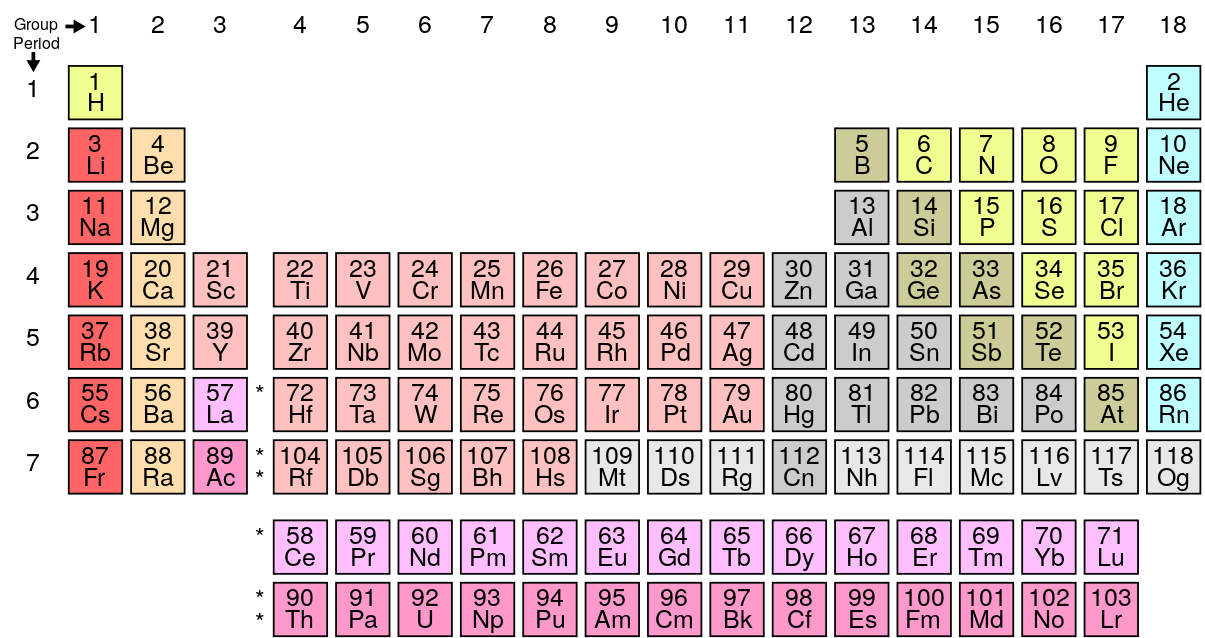
\includegraphics[width=\linewidth]{normal.png}
  \textit{Source: Offnfopt (Wikimedia Commons)}
\end{center}

The 118 known chemical elements are sorted into rows and columns,
where reading the table by rows yields the elements in order of atomic number
and the elements in a given column share chemical properties.
Each row terminates in a noble gas,
an atom whose outer electron shell is filled.
Since these shells grow in capacity in their filling order,
the rows of the table become progressively longer.
The row lengths, AKA periods, are 2, 8, 8, 18, 18, 32, and 32.
The last two rows are often, as above, interrupted
into two segments totaling 18 elements, which are placed with the rest of the table,
and a segment of 14, which is placed below it.
(These segments of 14 are the lanthanides and actinides.)
Without interruption, the table looks as follows.

\begin{center}
  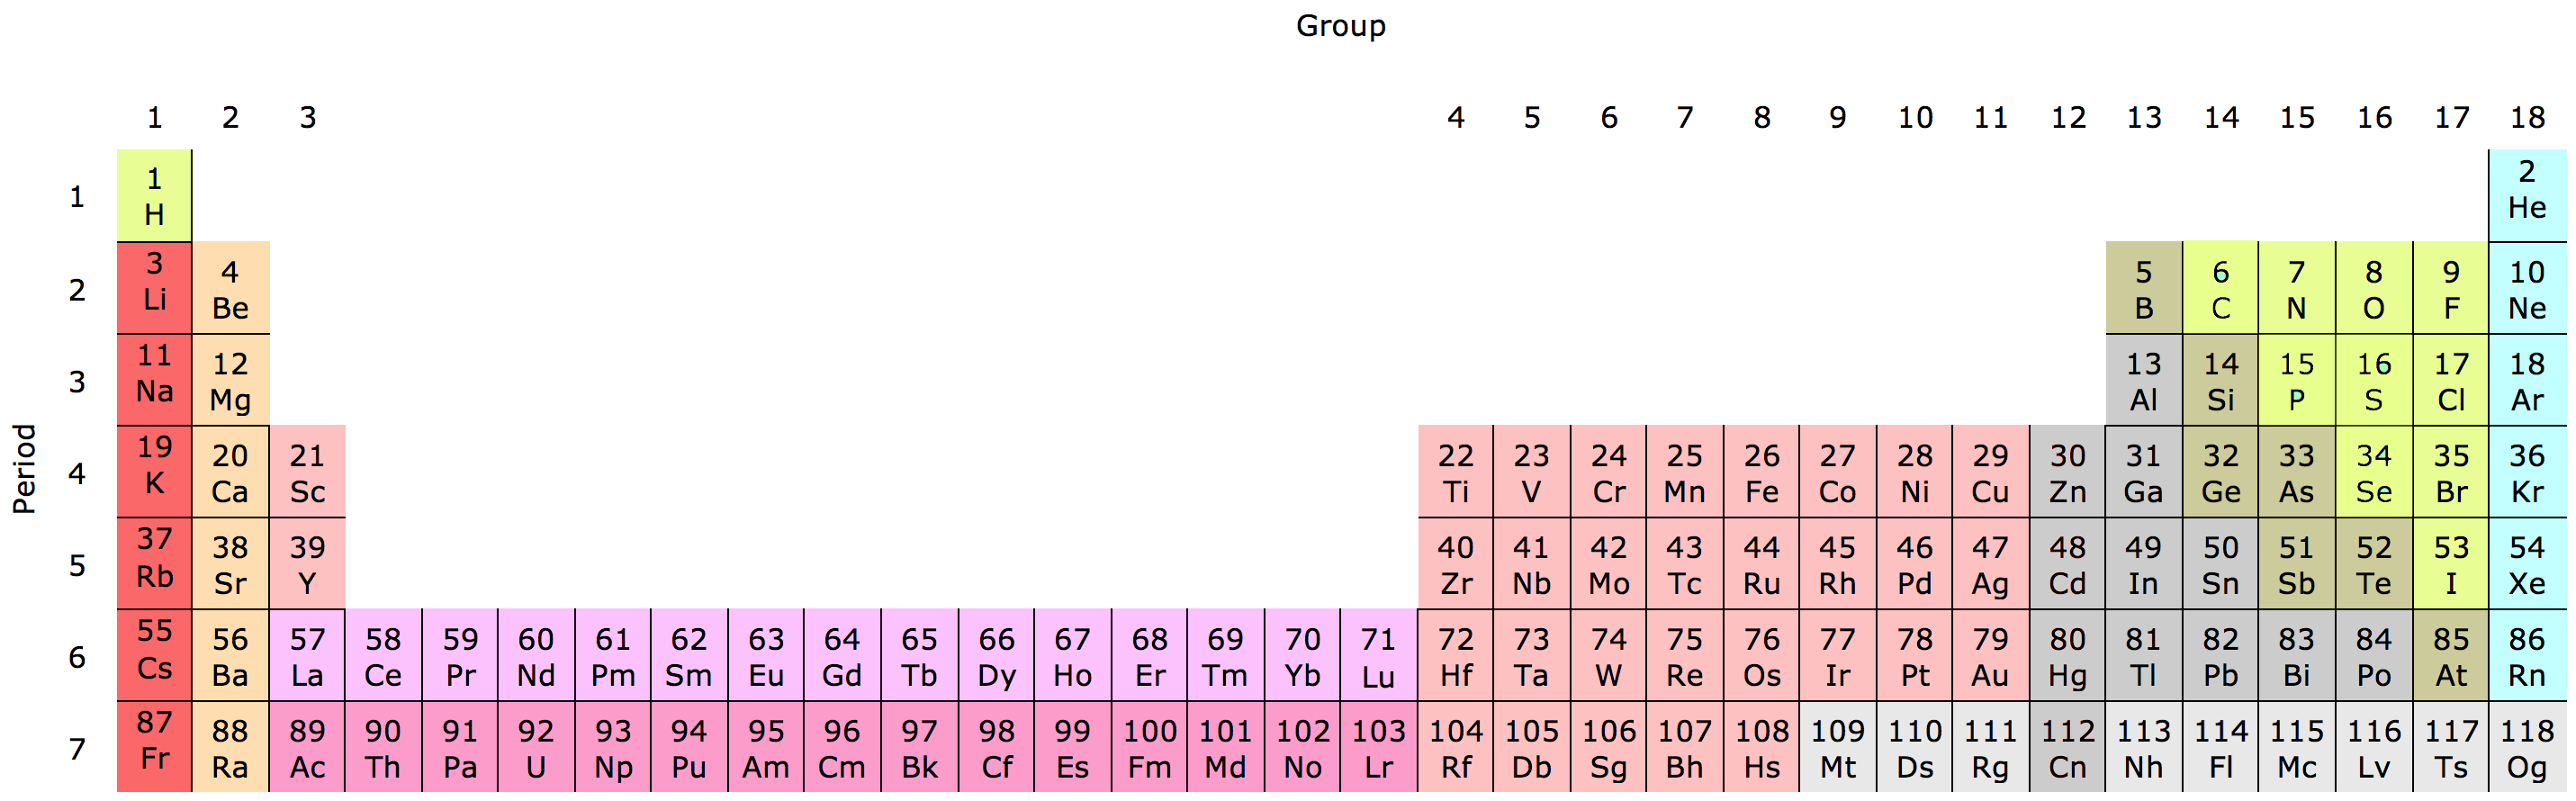
\includegraphics[width=\linewidth]{long.png}
  \center{\textit{Source: Sandbh (Wikimedia Commons)}}
\end{center}

But, where do the period lengths come from?


The answer has to do with the solutions to the Schr{\"o}dinger equation,
which are described by the four quantum numbers (QNs).
Each quadruplet of QNs represents a potential state of an electron orbiting the nucleus.
The numbers and their constraints are as follows:

\begin{center}
  \begin{tabular}{|c c c c|}
    \hline
    Name & Variable & Constraints & \# of values \\
    \hline
    Principal QN & $n$ & Integer, $0 < n$ & $\infty$ \\
    Azimuthal QN & $\ell$ & Integer, $0 \leq \ell < n$ &  $n$ \\
    Magnetic QN & $m_\ell$ & Arbitrary & $2\ell+1$ \\
    Spin QN & $m_s$ & Arbitrary & 2 \\
    \hline
  \end{tabular}
\end{center}

A pair of $n$ and $\ell$ describes a subshell of electrons,
and $m_\ell$ and $m_s$ index an electron within that subshell.
A subshell is written with $n$ followed by a letter based on $\ell$:

\begin{center}
  \begin{tabular}{|c|c c c c|}
    \hline
    $\ell$ & 0 & 1 & 2 & 3 \\
    Letter & s & p & d & f \\
    \hline
  \end{tabular}
\end{center}

For example, the subshell where $n=2$ and $\ell=1$ would be written ``2p.''
The potential subshells as given by the constraints are as follows:

\begin{center}
  \begin{tabular}{|c|c c c c c|}
    \hline
    n,$\ell$ & 0 & 1 & 2 & 3 & \ldots \\
    \hline
    1 & 1s & & & & \\
    2 & 2s & 2p & & & \\
    3 &3s & 3p & 3d & & \\
    4 & 4s & 4p & 4d & 4f & \\
    \vdots & \vdots & \vdots & \vdots & \vdots & $\ddots$ \\
    \hline
  \end{tabular}
\end{center}

Note that the latter two QNs are arbitrary,
i.e. only the number of possible solutions matters.
Their usual values are
$-\ell \leq m_\ell \leq \ell$,
$m_s = \pm \frac{1}{2}$.
The periodic table proposed here, however, will use
$0 \leq m_\ell \leq 2\ell$ and $m_s = 0$ or $1$,
for reasons that will become clear later.

Starting from hydrogen,
each element has one more proton than the last,
so each also has one more electron, assuming the atoms are neutral.
An atom attempts to minimize the total energy of its electrons,
so in general, the sequence of electrons added as the atomic number increases
is ordered from least to greatest energy.
Since the electrons in each subshell have very similar energy,
they fill up in a certain order,
where a subshell is completely occupied before the next one starts filling
(for the most part).
This order is dictated by the Madelung rule,
which states that the subshells are ordered first by $n+\ell$ in increasing order,
and next by $\ell$ in decreasing order.
This corresponds to traversing the triangle above
by diagonals sloping down and to the left.
The first few shells to be filled are:

\begin{tabular}{|c|c c c c c c|}
  \hline
  Subshell & 1s & 2s & 2p & 3s & 3p & 4s \\ 
  $n+\ell$ & 1 & 2 & 3 & 3 & 4 & 4 \\ 
  $\ell$ & 0 & 0 & 1 & 0 & 1 & 0 \\
  \hline
\end{tabular}

Each subshell is split into two halves based on $m_s$,
the spin of the electron,
which may be either up or down.
Since pairs of electrons with opposite spin have higher energy,
they are avoided for as long as possible.
This means that the halves of the subshell fill up in order,
e.g. all of the spin-up electrons are occupied before any of the spin-down ones are.
This is known as Hund's rule or the bus rule,
reflecting that passengers on a bus avoid sitting next to each other,
so every seat is occupied by one person before any seat is occupied by two.
Thus $m_s$ takes the next priority in ordering electrons.
Finally, $m_\ell$ serves to distinguish electrons within each half-shell,
so it is the final number used to determine the order in which shells fill up.
$m_\ell$ may take on $2\ell+1$ possible values,
so each subshell has twice that number of electrons.

With this knowledge in hand, we can begin designing a periodic table
which accurately reflects these rules
and makes determining electron configurations easy.
The rows of the conventional periodic table
correspond roughly but not exactly to all electrons of a given $n+\ell$;
the next row begins two elements before it is expected to,
placing the two columns corresponding to new electrons in s subshells
(known as the s-block) on the left.
There are advantages to this arrangement of the table,
particularly the existence of periodic trends,
where quantities like size strictly decrease as one moves to the right.
However, for the sake of mathematical idealism,
we can make each row correspond to a single value of $n+\ell$
while preserving the top to bottom, left to right order of the elements
by moving the s-block to the right side and one unit up.
This yields the left-step periodic table,
which was proposed by Charles Janet in 1928.

(Image)

However, like the long table,
the length of the rows increases quadratically as you move down,
since the difference between every row and the next (or rather, every other row)
is determined by the size of the new value of $\ell$ which becomes available.
As a result, the aspect ratio is very high,
making it inconvenient to display if width is limited,
and the problem will only become worse as new elements are discovered.
Preferably, the table should keep its shape in the long run as more elements are added.

\begin{enumerate}
\item $n+\ell$, increasing
\item $\ell$, decreasing
\item $m_s$, arbitrary
\item $m_\ell$, arbitrary
\end{enumerate}

\begin{center}
  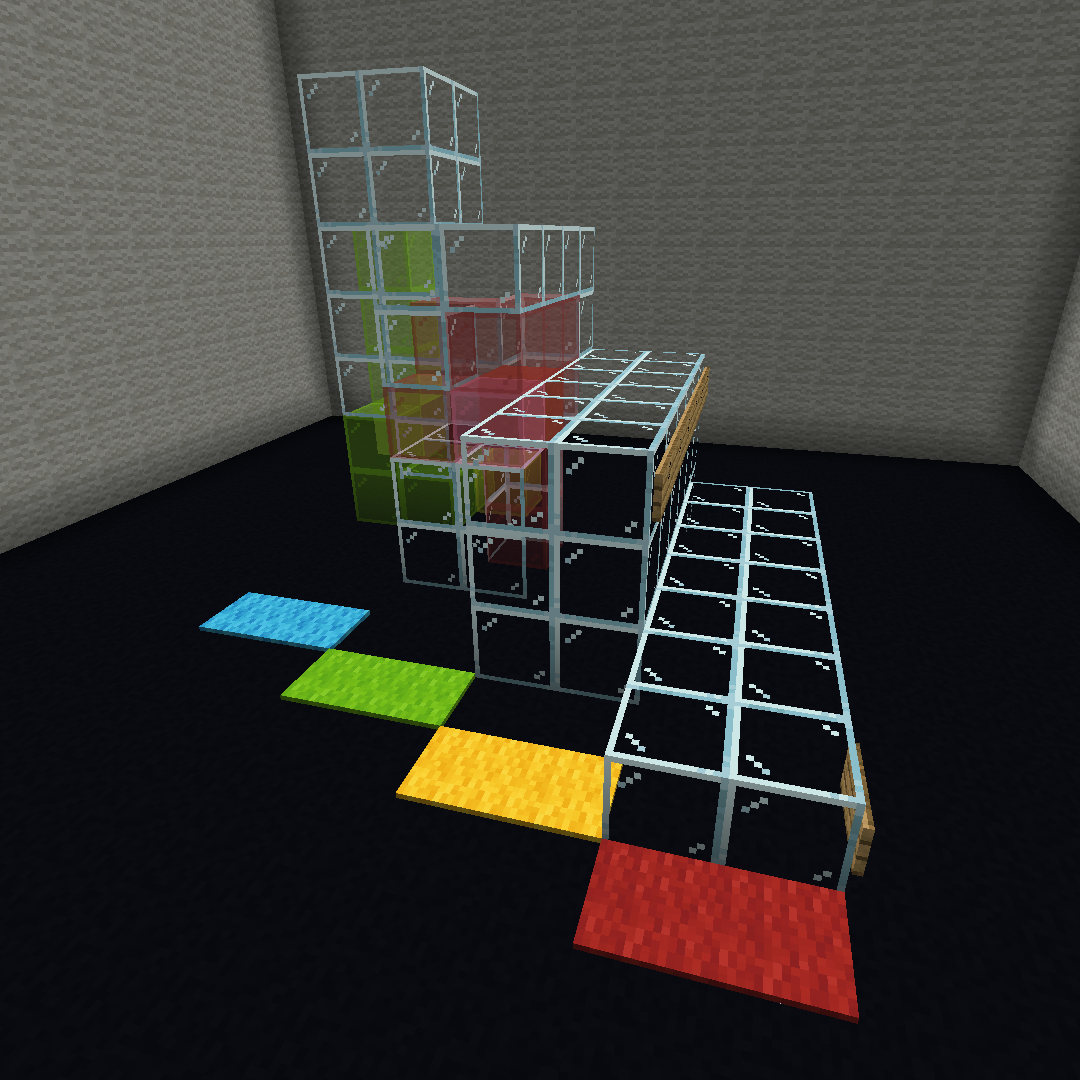
\includegraphics[width=0.5\linewidth]{mc1.png}
\end{center}

\begin{enumerate}
\item $n+\ell$, increasing, front $\rightarrow$ back (Madelung rule)
\item $2\ell+m_s$, decreasing, left $\rightarrow$ right (Hund's rule)
\item $m_\ell$, arbitrary, bottom $\rightarrow$ top
\end{enumerate}

\newpage

h

\end{document}
